\documentclass[12pt]{article}% \usepackage[utf8]{inputenc}
\usepackage{xcolor}
\usepackage{amsmath}
\usepackage{multirow}
\usepackage{graphicx}
\usepackage{subcaption}
\usepackage{wrapfig}
\usepackage[top=2cm, bottom=2.5cm, left=2.8cm, right=2.8cm]{geometry}
% \usepackage{minted}
\usepackage{natbib}
\bibliographystyle{plainnat}
\usepackage{cleveref}

% The following parameters seem to provide a reasonable page setup.

\topmargin0.0cm
\oddsidemargin0.2cm
\textwidth16cm
\textheight21cm
\footskip1.0cm

%The next command sets up an environment for the abstract of your paper.

\newenvironment{sciabstract}{%
    \begin{quote} \bf}
        {\end{quote}}

% Include your paper's title here

\title{Rapid dynamics in the retina}

% Place the author information here.  Please hand-code the contact
% information and notecalls; do *not* use \footnote commands.  Let the
% author contact information appear immediately below the author names
% as shown.  We would also prefer that you don't change the type-size
% settings shown here.

\author{Baptiste Lorenzi\\
    \\
    \normalsize{CentraleSupélec, Unversité Paris Saclay, Institut de la
        Vision}\\}

% Include the date command, but leave its argument blank.

\date{}

%%%%%%%%%%%%%%%%% END OF PREAMBLE %%%%%%%%%%%%%%%%

\begin{document}

% Double-space the manuscript.

\baselineskip24pt

% Make the title.

\maketitle

\begin{abstract}
    Retina ganglion cells extract visual information from natural scenes.
    Not only can they extract spatial patterns but also temporal patterns
    thanks to diverse adaptation mechanisms.
    It is unclear how these mechanisms are active under natural scene
    simulation. Here we trained a convolutional neural network (CNN) model on
    large-scale
    functional recordings of RGC responses to natural mouse movies, and then
    used this model to investigate the role of past visual events in the
    activity of
    retinal ganglion cells.
    Our work showcases how a combination of experiments with natural stimuli
    and computational modeling allows the discovery of novel types of stimulus
    selectivity and
    build some hypotheses on how they are implemented.
\end{abstract}
\textit{During my internship in Olivier Marre's team at l'Institut de la
    Vision, I am
    focusing on computational modeling of the retina. Olivier Marre's team is
    an
    interdisciplinary laboratory, hosting four professors and a dozen of
    interns,
    Ph.D. students and post-docs, working hand in hand to advance research
    on the retina. They all have various backgrounds mainly from biology,
    theoretical physics and engineering. In the context of this project, I've
    been
    working
    closely with Samuele Virgili, a third-year Ph.D. student, whose previous
    and
    current projects all focus on the modeling of retinal ganglion cells.}
\textit{I would like to thanks Olivier and Samuele for their kind supervision
    as well as the whole team for their
    warm welcome.}

\section{Introduction}\label{sec:introduction}

During my internship in Olivier Marre's team at l'Institut de la Vision, I am
focusing on computational modeling of the retina. Olivier Marre's team is an
interdisciplinary laboratory, hosting four professors and a dozen of interns,
Ph.D. students and post-docs, working hand in hand to advance research
on the retina. They all have various backgrounds mainly from biology,
theoretical physics and engineering. In the context of this project, I've been
working
closely with Samuele Virgili, a third-year Ph.D. student, whose previous and
current projects all focus on the modeling of retinal ganglion cells.

% Context
The ability of the visual system to process complex stimuli on different
temporal and spatial scales is remarkable. % Of which specie? 
Natural environments are such complex stimuli, and extracting the relevant
features at all times is crucial for many species.
% Here I already insist on two notions: natural stim and temporal complexity

Different neurons at different stages of perception are sensitive to specific
features of the visual stimulus. From a theoretical point of view, the retina
doesn't only play the role of a receptor for the visual system. It has been
proven to be the first layer of feature-sensitive
neurons \cite{gollisch_eye_2010}.

Both the accessibility and apparent complexity	of the retina makes it a
perfect candidate for the study of the front-end of visual processing
\citep{gollisch_eye_2010}. In the mouse, the retina is composed of more
than 30 parallel feature channels, embodied by ganglion cell types. Through
their axons, the optic nerve, they provide information to numerous visual areas
in the brain.
A few channels are active in the encoding of basic features including luminance
changes and motion, that are only combined in more downstream area. Other
channels however are known to play a role in the extraction of specific
features of natural scene that are relevant  to behaviour.
% This example focusing on behaviour is not the best one here...

Still, we currently lack an explanation of the features extracted by other
channels. One of the historical reasons for this is that synthetic stimuli used
to study retinal responses are not complex enough to activate these channels.
Hence, they cannot uncover critical response properties encountered in natural
environments. % Please rewrite this sentence

% Here add an example of how synthetic stimuli have been used to study adaptation

In practice, Karamanlis and colleagues \citep{kim_nonlinear_2020} have
probed a larger complexity in retinal spatial non-linearities thanks to stimuli
capturing the statistics of natural environments.
As those non-linearities cannot be captured by Linear-Nonlinear (LN) models,
convolutional neural networks (CNNs) have become the state-of-the-art approach
for predictive modelling of visual processing, not on;y in the retina but also
in higher visual areas. % Now briefly explain one or two studies that used CNNs to study adaptation

\textbf{Insight on methods}
Here, we combined the power of CNN-based modelling with large-scale
mutli-electrode recordings from RGCs to investigate the mechanisms of fast
adaptation in the retina under natural stimulus conditions. To this end, we
recorded RGC responses to flashed images paired together. Each pair is composed
of a synthetic adaptation image followed by a natural image. We were able to
identify different trend in the responses of RGCs to natural images, depending
on the adaptation image.

To investigate the diversity of this adaptation process and its implementation,
we paired deep convolutional models with more traditional modeling. We trained
a CNN model on RGC responses to a movie of flashed images. After training, we
study how the how this model generalized to images after being adapted with
patterns it wasn't trained to. By tweaking part of the model at the inference
level, We hope to show that temporal mechanisms such as gain-control play a
major role in the fast adaptation of RGCs in a natural context.
\section{Background}\label{sec:background}

\textbf{The retina.}
In vertebrates, the retina is part of the central nervous system. It consists
of just a few layers of neurons, each with a distinct role in processing visual
information (Figure \ref{fig:retina_structure}, Left).

\begin{figure}[h]
    \centering
    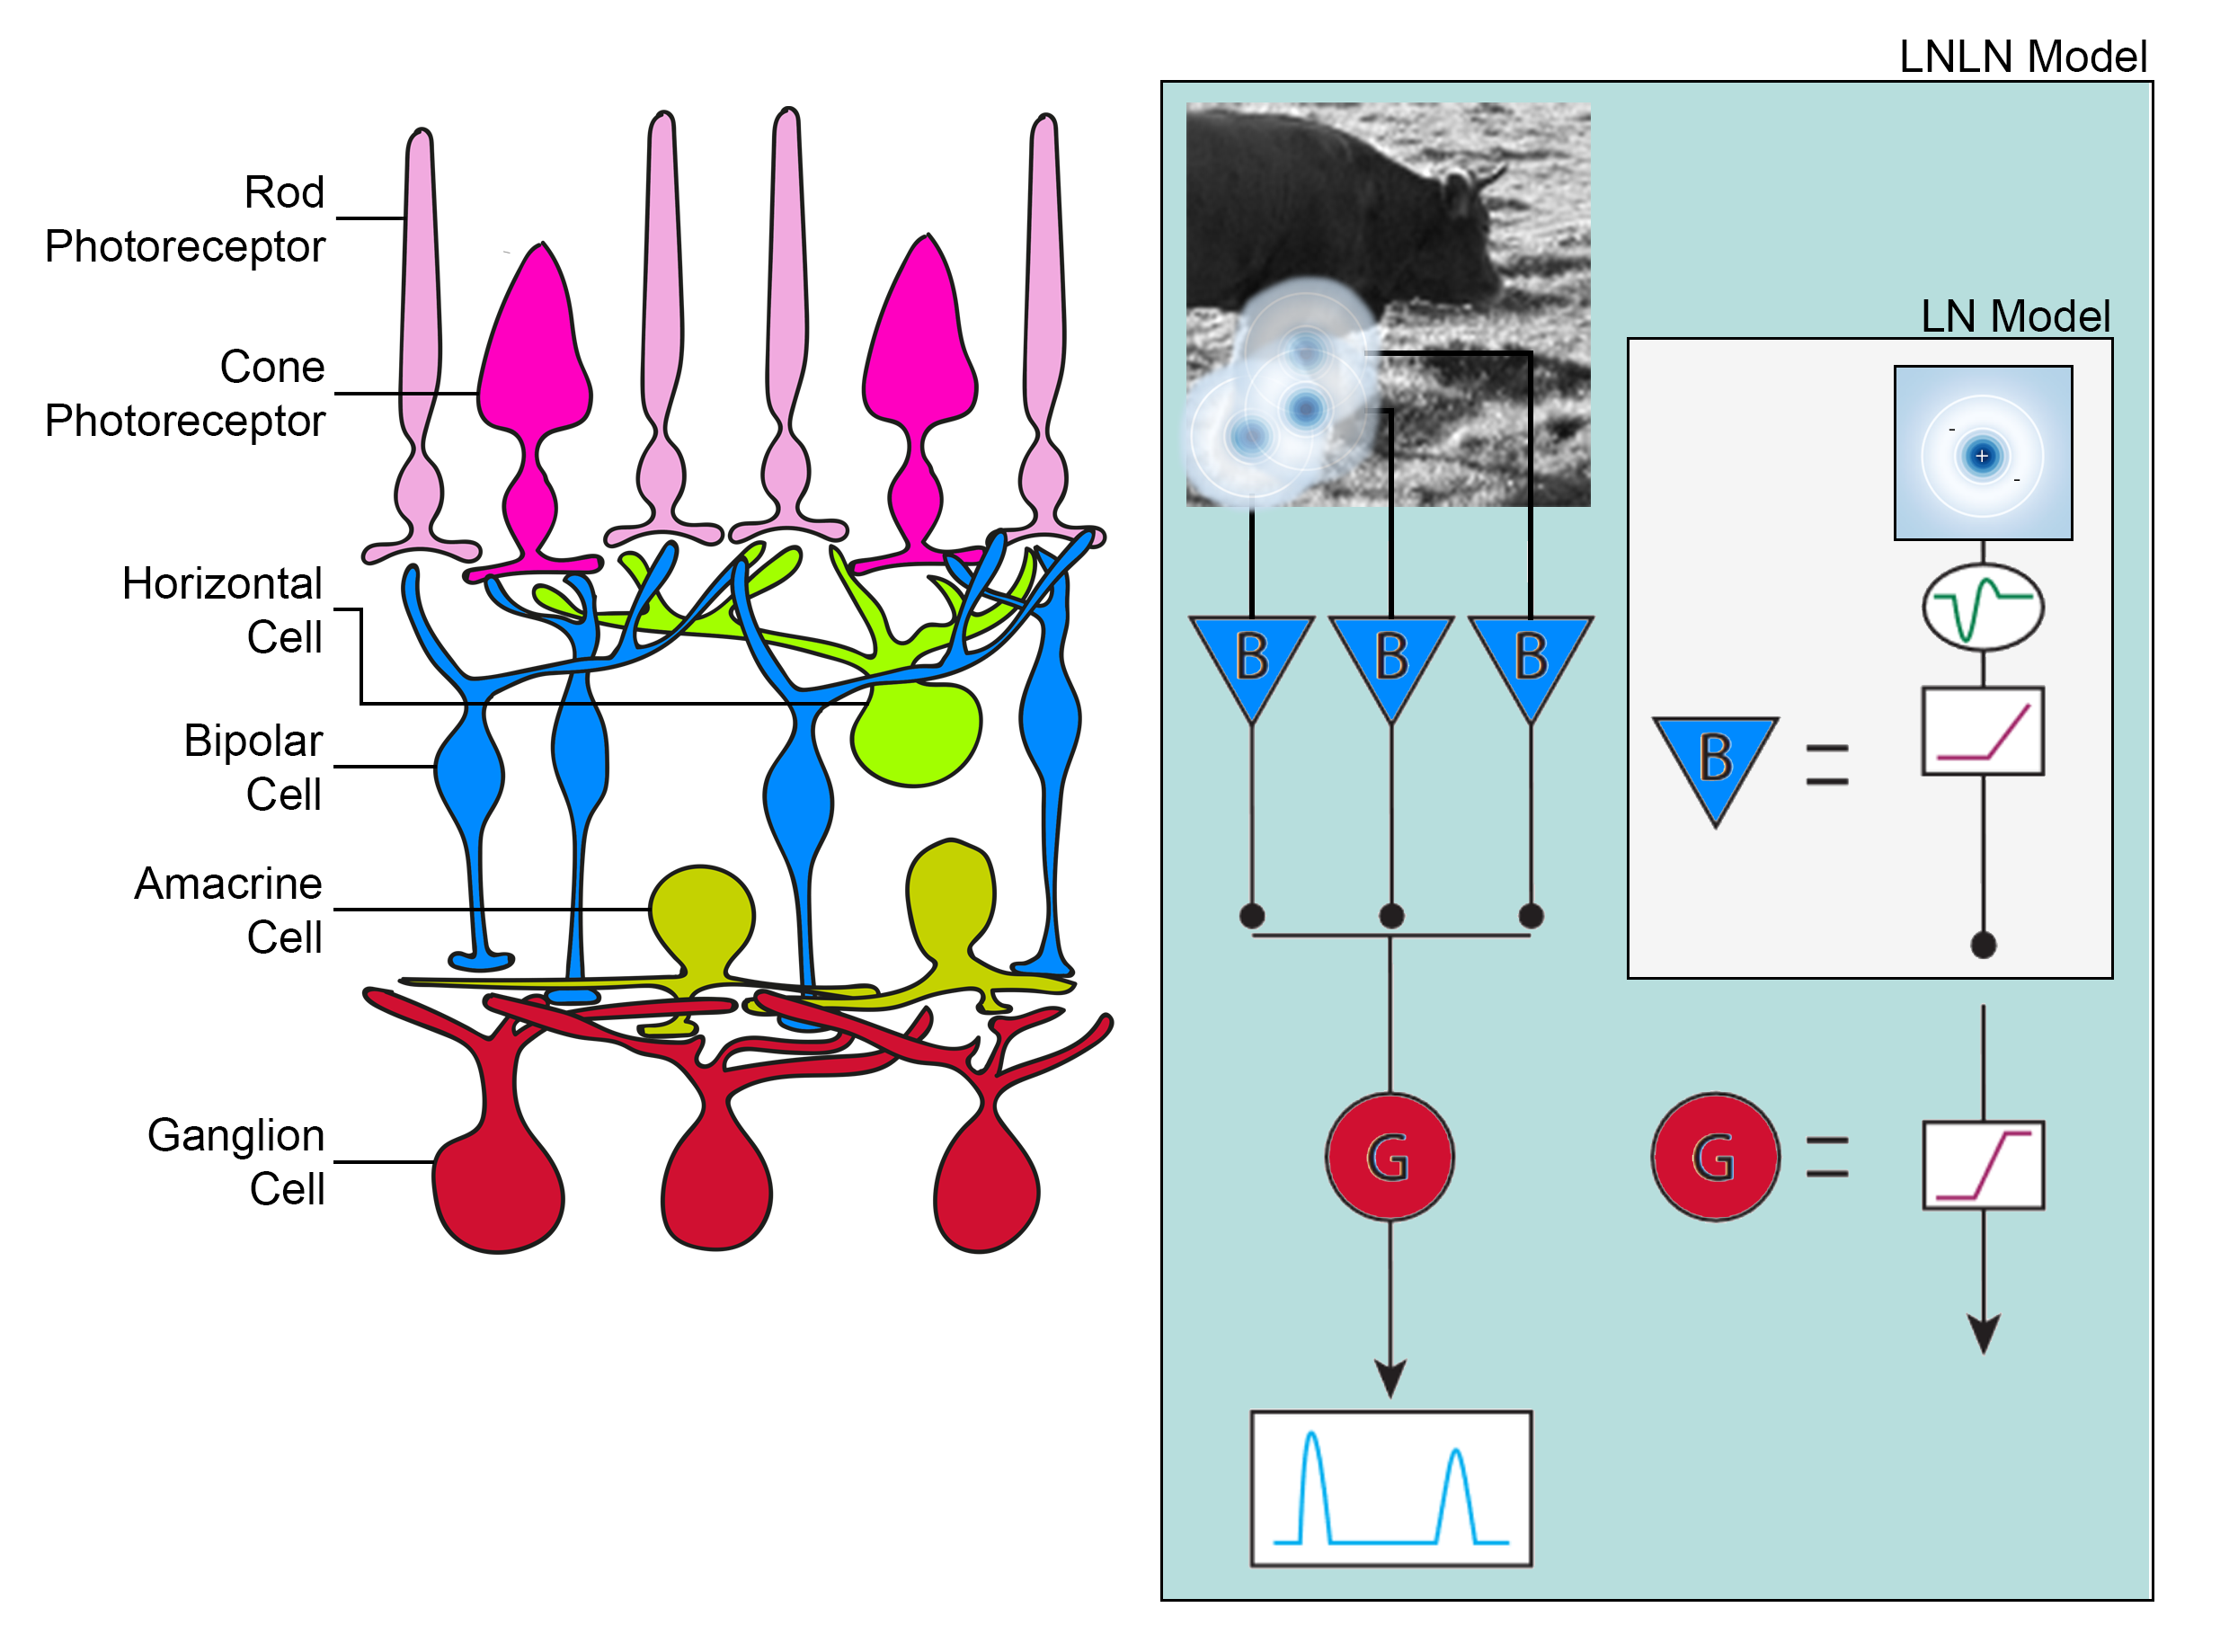
\includegraphics[width=\textwidth]{pics/RetinaAnatToFunction.png}
    \caption{\textbf{From anatomy to functional modeling.} \textbf{Left.}
        Schema of the layered anatomy of the retina. \textbf{Right.} Schema of
        a LNLN
        model. In standard LN
        models,
        photoreceptors are considered purely linear and simply mapped to each
        pixel of
        the visual input. Bipolar cells tile the input space. They are modeled
        as a
        spatial linear filer, a difference of Gaussian defining an excitatory
        center and
        inhibitory surround, a biphasic linear temporal filter and a
        non-linearity.
        Ganglion cells pull and average the signal from all the bipolar cells
        in
        their
        receptive field, and spike selectively depending on their
        non-linearity. Notice the simplicity of LNLN model compared to the
        anatomical
        description of the retina.}
    \label{fig:retina_structure}
\end{figure}

At its forefront are photosensitive neurons known as photoreceptors, which
serve as the initial light sensors within this neural network. Rods are for
low-light
and peripheral vision, while cones are for bright light, color perception, and
central vision. Rods are more sensitive to light but don't perceive color,
while cones enable color vision.

These photoreceptors stimulate bipolar cells, a diverse group comprising 15-20
anatomical
distinct types in the mouse. They all exhibit unique
responses to visual stimuli, with an even larger functional complexity than
anatomical diversity. % Functional/genetic/anatomical types?

The bipolar cells, in turn, excite retinal ganglion cells (RGC) which then
transmit the pre-processed visual  information to the rest of the
brain via the optic nerve.
RGC of the same type are described as sharing the same
physiology morphology,
intra-retinal connectivity, retinal mosaic and genetic markers. It is not yet
known if such biological markers are enough to define the variety of functional
output channels of the retina. According to Baden and co-workers, there should
be at least 32 different RGC
functional types \citep{baden_functional_2016}. An example of functional
diversity in the RGC groups is their preference for local light increase and/or
decrease. They are respectively referred as ON, OFF and ON-OFF RGC.
Furthermore, different species have different sets of RGCs whose parameters are
influenced by evolution.

Additionally, the retina hosts two families of inhibitory neurons: horizontal
and
amacrine cells. These neurons play a crucial role in modulating the activity of
excitatory cells, adding another layer of complexity to the visual processing
within the retina.

Compared to the rest of the brain, the retina is relatively simple,
making it an ideal neural tissue for in-depth study using computational models.
Its accessibility for experimental research further enhances its appeal as a
valuable subject for investigating neural code and neural processes.
% I guess the figure is enough

\textbf{Adaptation in the retina}
To operate optimally in a wide range of
stimulation conditions, the retina adapts its responses to the statistics of
the visual scene.
In particular, it was observed to adapt to the average
luminance as well as the range of intensity fluctuations about the mean,
referred to as the contrast of the scene.

Visual systems can function over a wide range of light intensities, from
starlight to a bright sunny day – a luminance range of $10^{10}$.
At first glance, the retinal adaptation to the luminance of the scene is quite
simple by nature.
For instance, it is known that the retina uses different neuronal
pathways at low and high luminance. Rods and their retinal neuronal channels
cover the dimmest light while cones facilitate contrast, color and motion
discrimination but only in brighter light.

%clear, need proof
In a high-contrast environment, RGC tends to be much less sensitive than
in low contrast environment. %FIND SOURCE
This sensitivity adaptation happens on different timescales.
A large change in stimulus contrast wouldn't change the response properties of
cones and horizontal cells \citep{baccus_fast_2002}. But it would change the
behavior of
bipolar cells, meaning fast adaptation to contrast begins in their sublayer.
This almost immediate effect of a contrast increment changes the properties
of some bipolar cells, including their temporal patterns as well as their
selectivity. Their diverse response to this contrast increment
is correlated to the diversity of functional and morphological subtypes among
bipolar cells.
Interestingly, This evolution is also seen in all ganglion cells.

% ADD MORE DETAILS ???

% In the paper, there is an Intersting passage on modeling that could be useful here

Furthermore, contrast adaptation happens primarily in a global manner overall
the receptive field of a ganglion cell.
Garvert and colleagues stimulated different parts of the receptive field of one
ganglion cell with either the same light intensities or changing light
intensities \citep{garvert_local_2013}.
Surprisingly, when the light level changes in the second area, the response in
the first area where light did not change was more impacted in comparison.
Not only does this show that contrast adaptation happens on a scale smaller
that the receptive field, it also describes this adaptation as being complex to
apprehend.
The local nonlinearities in the neuronal pathway leading to the ganglion cell
response should be responsible for this effect \citep{schreyer_nonlinear_2021}.

Local contrast adaptation is especially relevant in
understanding how ganglion cells respond to natural images since these stimuli
are full of spatial details like edges in which two contrast levels appear
simultaneously. Such images are challenging to use, as they can't be summed up
to a few statistics easily.

% Here, I want to cite the global and local adaptation paper and inisist on the stimuli they used

\textbf{Retinal response to natural images.}
Most of the knowledge we have on the retinal response comes from experiments
using synthetic stimuli that don't reflect the full diversity of natural
scenes that the mouse retina evolved to respond to. In
\cite{goldin_context-dependent_2022} showed that the
aforementioned ON-OFF selectivity of RGC is maintained under natural scene
stimulation. By recording how RGC respond to natural images perturbed by
random noise patterns, they were able to measure the local selectivity of RGCs
to natural stimulation.
Thanks to that method, they were able to show that the selectivity of RGCs
depends on the image. Another interesting aspect of their work is that with
careful modeling using convolutional neural network modeling, they have shown
that this resulted from the non-linear combination of diverse pathways in the
retina. In particular, ON-OFF selectivity seems to be encoded by the contrast
of the image, revealing the retina to extract more complex features from the
retina than previously thought.

\textbf{Standard model of the retina.}
Two standard functional models of the retina have been used with
great success. The simpler model, the Linar-Nonlinear (LN) model, describes a
functional unit
of the retina as a combination of a spatio-temporal linear filter and a
non-linearity (Figure \ref{fig:retina_structure}, Right).
The Linear-Nonlinear-Linear-Nonlinear (LNLN) model, models a RGC as a cascade
of LN models representing bipolar cells.

\textbf{Convolutional Neural Networks.}
Due to the large statistical complexity of natural scenes, convolutional neural
networks have grown to be a new standard for modeling retinal responses to
natural images. However, compared to baseline models, they tend to be harder to
read from a biological perspective. Hence there is an ongoing debate in the
field on the limitations of those models in the context of the study of the
retina. We believe that with careful modeling decisions, it is possible to
learn a lot from those models, especially regarding local and temporal
dynamics.

CNNs have also been used to describe the cortex response to natural images
\citep{cadena_deep_2019}. The amount of available cortex data even led to the
development of a 'foundation model' of the mouse visual cortex with a
remarkable capacity to generalize to various stimulus domains
\citep{wang_towards_2023}.

While CNNs modeling prowess can be measured using traditional metrics such as
their ability to predict the average spiking rate response of a ganglion cell
to a given image, it's hard to pinpoint what is missing in their predictions.

\clearpage
\section{Methods}\label{sec:methods}

This work is in some ways a continuation of
\cite{goldin_context-dependent_2022}, from which we derived most of the methods
presented here. By comparison, this time we take account of temporal dynamics
in the responses. The switch from 2D visual inputs to 3D spatio-temporal inputs
complexifies every steps of the analysis but is ... COMPLETE

\textbf{Retinal recordings.}
Since I don't realize any experiments myself, I will try here to give as few
details
as necessary for the understanding of the rest of the work. Still, experimental
recording of the retina is a very interesting topic and the reader can look
here for more information. % Useful ?
The laboratory has access to three experimental rooms that enable
state-of-the-art experimentation
on the retina.	For this project, we record the activity of retinal ganglion
cells
using a multi-electrode array. The retina is placed on a ???
% TO COMPLETE

% A part to complete

\textbf{Stimuli design.}
The stimuli used in this project are composed of two images, one synthetic
adaptation image followed by a natural image. Adaptation images are taken from
a pull of three different patterns: a grey screen used as control, a
checkerboard of X*X checks and the same checkerboard with inverted colors (Fig.
TO ADD). Natural images are taken from ADD REFERENCE. XXXX images were used for
training the CNN, 10 were used to test the CNN and among them, 3 were used to
record an estimation of the LSTA of each cell.
Adaptation and natural images are always paired together to form a single
stimulus pair, also referenced as a clip. Each frame is XXXxXXX pixels wide and
each clip is 2*400ms long.

% Give details about how the images are built for the camera?

The training set is composed of XXXX clips, each composed of the grey
adaptation image followed by a natural image. The test set is composed of 30
clips, each repeated 30 times. The test clips are composed of 10 different
natural
images preceded by each adaptation (3 different clips for each natural image).
The dataset used to record LSTA is composed of 9 different clips repeated 1000
times. Each clip is composed of one of the three selected natural images
preceded by one of the adaptation patterns.

We first used 4 different natural images while computing the LSTA of each cell,
each 12 different clips being repeated 12 times. We found that the estimation
of the LSTA was too unstable with only 750 repetitions. In following
experiments we excluded the image that yielded the least amount of stable
estimations of LSTA (20\% average success rate as compared to 42\% average
success rate for the other three images). We then used 3 different natural
images while computing the LSTA of each cell, each 9 different clips being
repeated 1000 times. We found that the estimation of the LSTA was stable with
1000 repetitions.

\textbf{Data processing.}
Multi-electrode array experimental data takes the shape of a collection of
temporal electrical signals tiling the recorded area.
In most scenarios, including here, these signals are sorted into different cell
signals using a semi-automatic algorithm. This algorithm is based on the shape
of the electrical spikes as well as their spatial location. It is
quite messy due to the low signal-to-noise ratio in the data and each
experiment
needs to have its sorting corrected by hand. This process can take up to an
entire day for a single experiment. I used spiking-circus for semi-automatic
spike sorting and the UI phy for handmade corrections. [CITE]
It is important to note that even though the retina is an easier organ than
most to record clean spike signals from, the data is still very noisy and the
sorting process is not perfect. Hence, when validating hypotheses, cells are
usually rated by their reliability.

% Checkeckerboards and RF
After spike sorting, we analyze the recording from standard stimuli to
characterize each
ganglion cell receptive field. To this end, we display a random binary
checkerboard for approximately 1 h at 30 Hz. Check size is 42\microns. A
ganglion cell receptive is computed as its spike trigger average (STA), for
this checkerboard stimulus. The STA of a cell can also be described as the
stimulus that triggers the most spikes from that cell. It is computed as the
average of the presented checkerboard weighted by the number of spikes using a
set number of samples per repetition (here 21). The spatial STA is usually
shown as the 2-dimensional spatial slice at the maximum value after smoothing.
Temporal STA is the one dimensional time slice at the pixel with the maximum
value. For smoothing, a double Gaussian is fitted on the resulting spatial
STA.

% Cell typing (probably useless here, but say a word about it)

% Nat images
\textbf{Natural images.}
We used a subset of the Open Access van Hateren Natural Images Dataset [ADD TO
        BIB]. It consists of monochromatic and calibrated (perfect mapping from
pixel
value to luminance) images of diverse natural environments. These images need
to
be preprocessed to avoid triggering the adaptation to different ranges of light
intensities in the retina, which would call unwanted
dynamics. First, images with numerous saturated pixels were not included in our
subset. Using a custom procedure previously developed in the laboratory, we
then
ensured the images were normalized in the mean luminance and the root mean
square (RMS) contrast.

\textbf{LSTA.}
To record the local specoficity of the response of a ganglion cell to a natural
image, we used a method called local spike trigger average (LSTA) for its
analogy with the STA. This method was previously developed in the laboratory.
We first generate a set of perturbed natural images by superimposing some of
the natural images (3-4 images) with various perturbation patterns in the form
of random checkerboards. We once again used a checker size of 42\microns.
Following calibration guidelines measures in previous experiments, the
amplitude of the perturbation was set to 12.5\%, where 100\% corresponds to a
pixel value of 1. In the mouse retina, this amplitude was found to trigger a
change in firing rate of approximately 1.5Hz in ganglion cells with high firing
rates to the unperturbed images \citep{goldin_context-dependent_2022}.

\textbf{Data visualization.}
Due to the diversity of the data we work with, it can be challenging to have
all the relevant information on one screen. First, it's important to always
have the rasterplot in sight since it informs of the quality of the cell at a
glance. I u

\textbf{Data selection.}
Not all recorded cells are suitable for all types of analysis. Overall, the
main
quality we look for in a cell is its stability during an entire stimulus clip.
It reflects its health and likeliness to behave normally during the
presentation. For our most complex experimentations, cells need to remain
stable in-vitro for up to five hours, which is quite unlikely. In Fig. , we
describe the different selection steps and their influence on the amount of
usable data.
Tp
% Graph idea : All type of rasters for one cell
% Bar chart representing the fading amount of data that can used for modeling

Blablable to share my programming skills to help and improve the data pipeline
of
the
laboratory.

% Models : Put the emphasis on the balance between G.C. and data-driven models
% Also insist on the time component of the models
\textbf{Modeling.} This should be the main part of my internship and also the
most challenging. We are designing a dynamical model of the retinal fast
adaptation. In fact, we mostly look at the evolution of the response from an
image to another, meaning that the dynamic we observe only spans two points in
time. This reduction makes the model more realistic to study. Most of this job
can be summarized as model design, python programming, sensitivity analysis and
data fitting. By comparing how different modeling strategies reproduce the
observed LSTA in the data, we can gain insight on how fast adaptation to
natural scene is implemented in the retina.
%I think what is missing here is what question you want to answer with this. We should discuss this more. 

Our baseline model is the LNLN model of ganglion cell widely used in the
literature. Each neuron is encoded as a spatial linear filter chained with a
non-linearity (usually an activation linearity in the like of ReLU). A single
layer of subunit neurons, representing bipolar cells, converge into a single
modeled ganglion cell.	We would like to add temporal dynamics to this model,
either by adding a time dimension to the spatial liner filter of the cells or
by considering a gain control mechanism. This last mechanism consists in
scaling up or down the present output depending on past outputs (Figure
TO FIND~\cite{}).

\begin{figure}
    \centering
    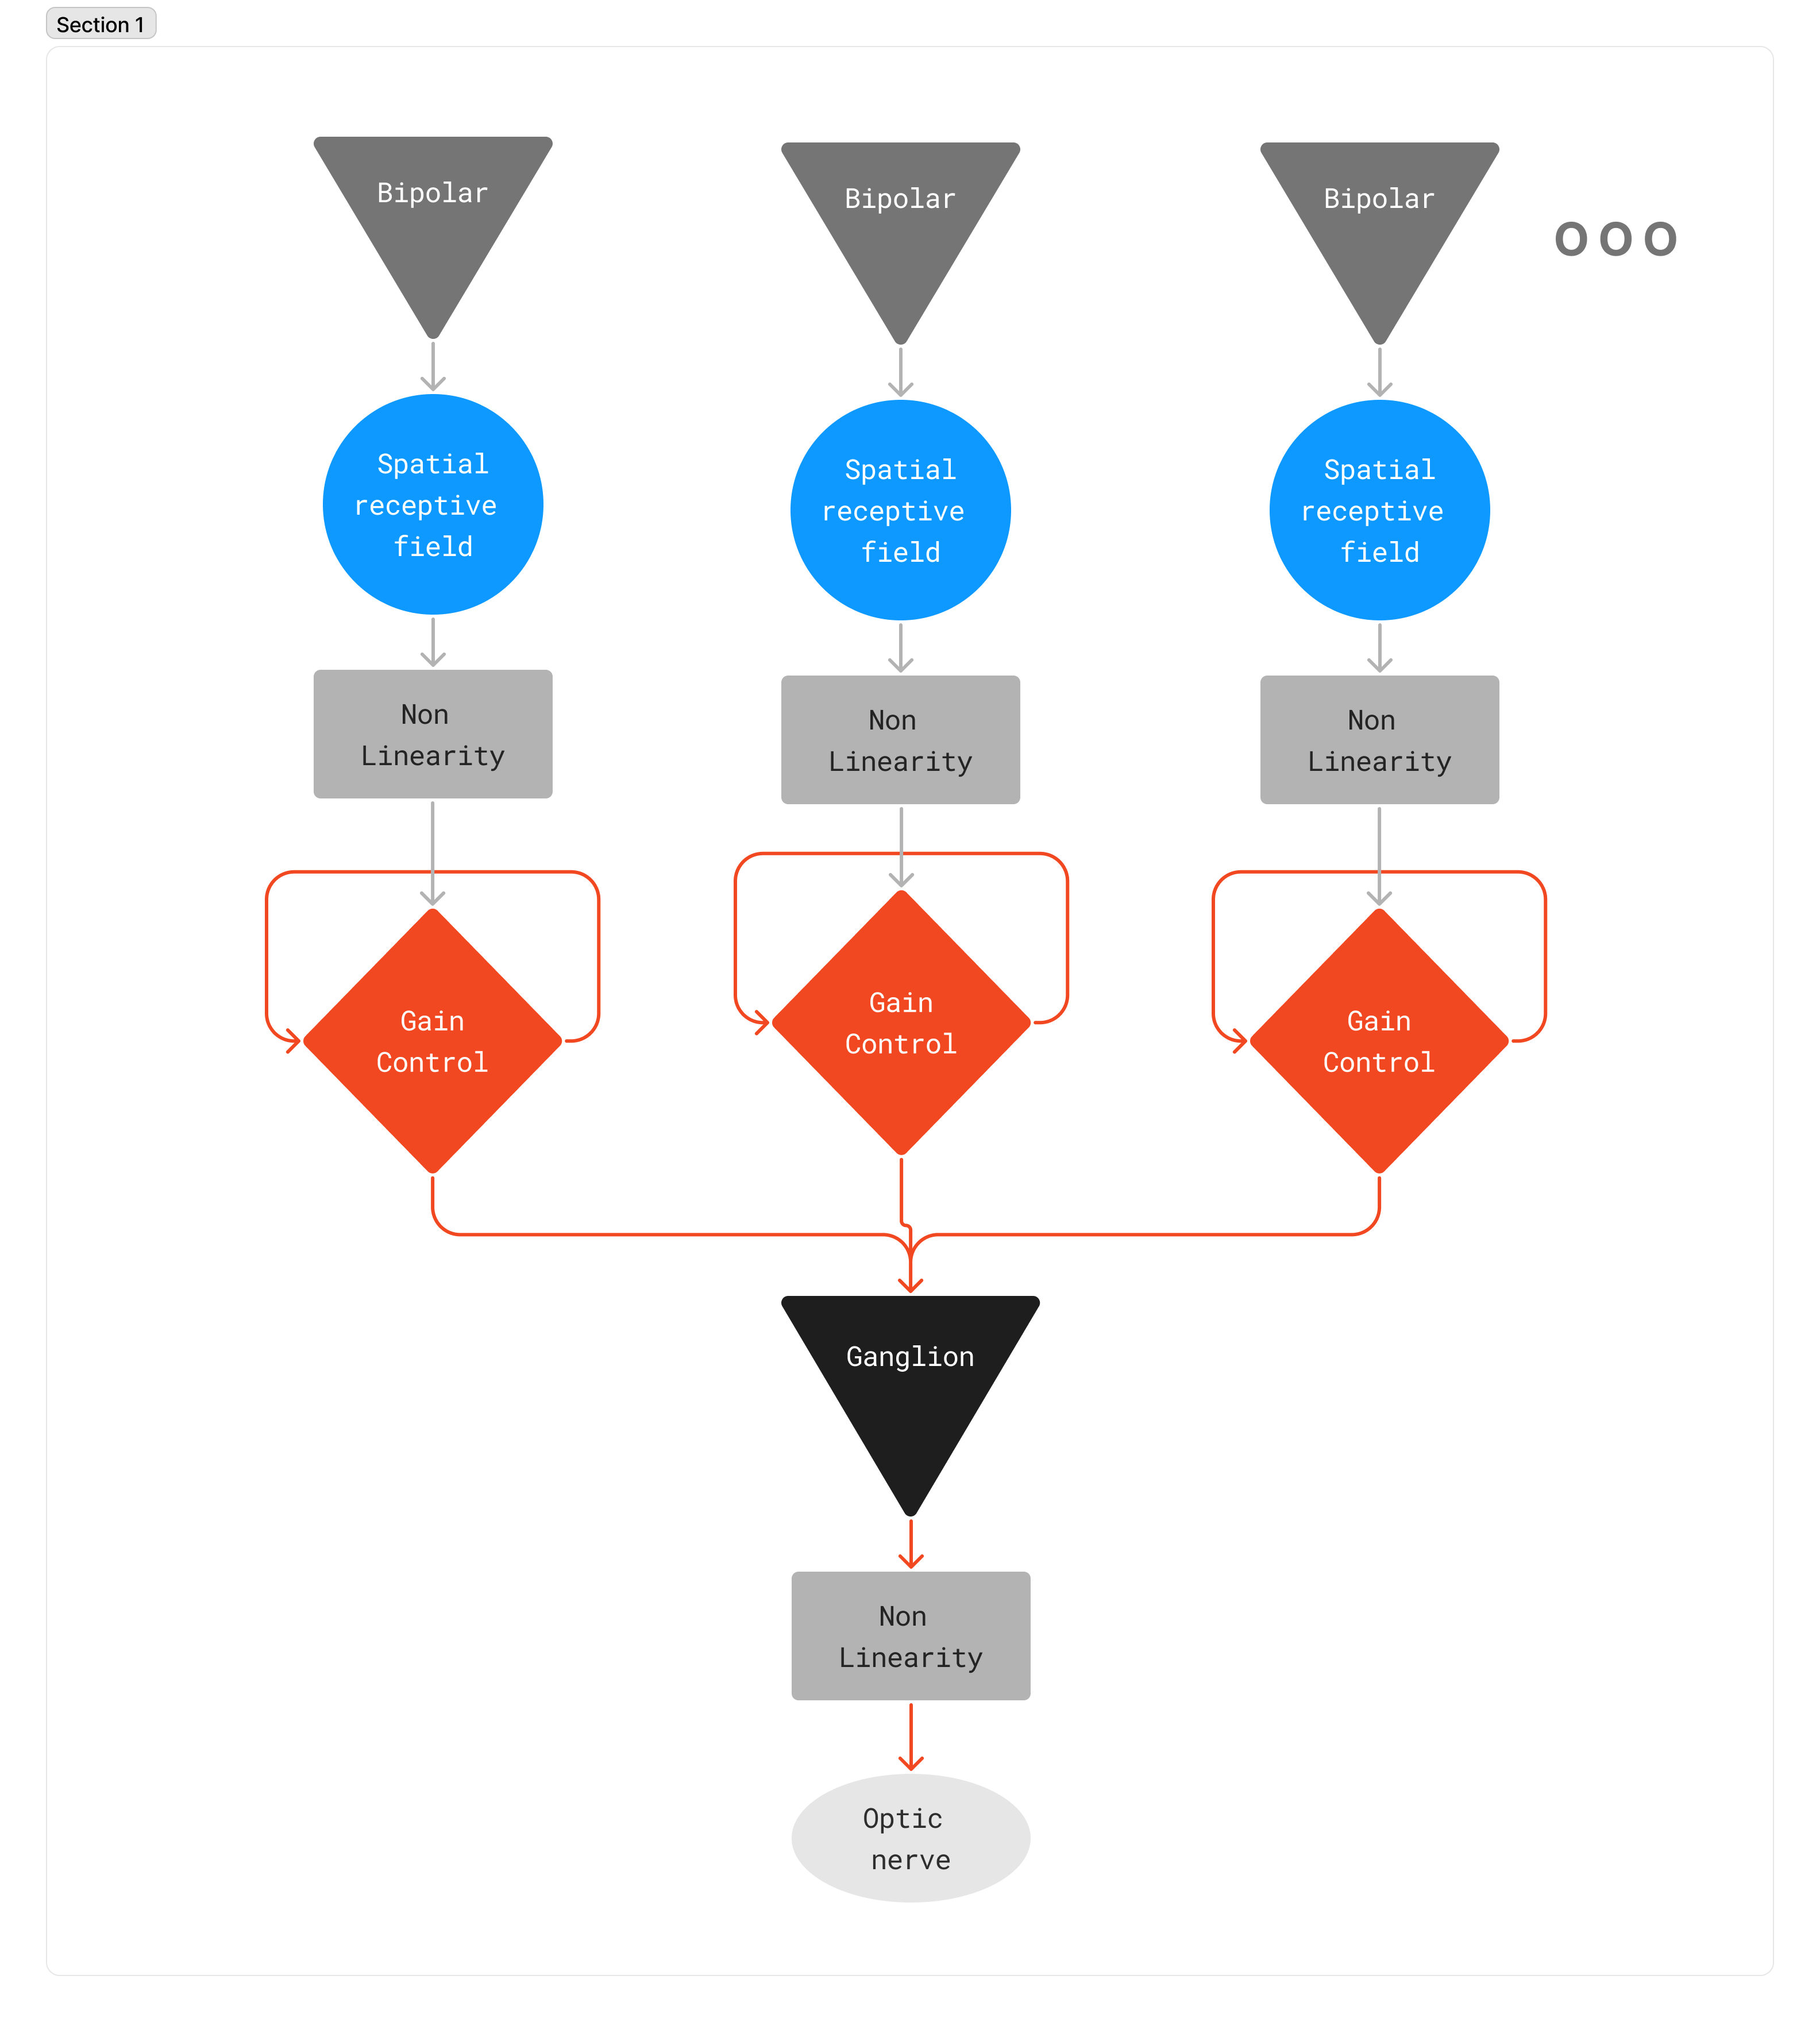
\includegraphics[scale = 0.2]{pics/GCModelDiagram.png}
    \caption{\textbf{Quick sketch of a gain control LNLN model.} Each bipolar
        cell is
        composed of a linear spatial filter that selectively responds to part
        of the scene,
        a non-linear activation function, and a gain control mechanism that
        scale its output
        depending on past events. They all converge into on bipolar cell
        (forming its receptive field)
        of which output is also modeled using a non-linear function.}
    \label{fig:LNLN}
\end{figure}
We will first study our models in a data agnostic manner and study its behavior
for different set of parameters. We will then fit it on our own experimental
data using an efficient optimization framework in python using strategies
developed in the field of machine learning.

\section{Results}
\label{sec:results}

Here, we investigated fast adaptation in the mouse retina under natural
stimulus conditions. To this end, we trained a CNN model on RGC responses to a
movie of flashed images appearing naturally in the mouse environment,
% and then performed a model-guided
% search for stimuli that maximize the responses of RGCs.

\textbf{A method to estimate how selectivity to natural images changes over
    time.}
We recorded retinal ganglion cells (RGCs) in the mouse retina with
multi-electrode arrays (MEAs) while displaying sequences of natural images.
Each image was presented for 400 ms, preceded by one of three 400 ms adaptation
light patterns: grey, checkerboard, or inverted checkerboard (Figure
\ref{fig:CellExample}).
Each pair of adaptation patterns and natural images forms a stimulus clip
lasting 800 ms.
To measure the selectivity of RGC to different parts of the image, we added dim
checkerboard patterns (Figure \ref{fig:LSTA}).
The amplitude of the perturbation checkerboard was selected to introduce a
small yet visible change in the RGC response compared to the RGC response to
the unperturbed natural image.

For each cell and each stimulus clip, we computed an estimation of the local
spike-trigger average (LSTA) (Figure \ref{fig:CellExample}), as the average of
the
perturbation patterns weighted by the number of spikes they evoked. This
estimation is similar to a more classical Spike Trigger Average (STA) but due
to the small amplitude of the perturbation checkerboard, we explore here a
small, local region of the stimulus space centered on the reference natural
image. The LSTA is a visualization of the gradient of the RGC response at the
reference natural image point in stimulus space. From an experimental point of
view, instead of perturbating the biological system itself (e.g. shutting down
neuronal pathways), we perturbated the stimulus itself.
1000 repetitions with different perturbation patterns were necessary to
estimate the LSTA to one clip (see Methods).

We recorded RGC responses from four different eyes. The first experiment was
discarded since 750 repetitions were not sufficient to estimate the LSTA. The
second experiment was also discarded since the retina was very unhealthy during
the recordings. The third experiment was a great success with over 100 cells
showing relevant LSTA for many different clips. Finally, we used a fourth
experiment to both train and test a convolutional neural network and measure
LSTA, once again with
great success with about 100 cells with LSTAs despite the longer experimental
time.

\par~\textbf{Ganglion cells can change their selectivity depending on previous
    light patterns.}
We looked at the firing rate and the LSTA of more than 200 cells changed
depending on the adaptation light pattern. Some clear hypotheses can be made as
described in Figure \ref{fig:CellExample}. Adaptation effects can already be
seen in the temporal profiles of the responses.

As for the spatial effect on the LSTA, a first hypothesis would be that for On
cells, an area that stays white provokes less response than an area that goes
from black in the
adaptation pattern to white in the natural image (Figure \ref{fig:CellExample},
On cell, column 1) - respectively black for
Off cells (Off Cell, column 2,3). However, this hypothesis does not hold true
in all cases (On
cell, column 3). For OnOff cells, this adaptation can happen in both pathways
simultaneously
(Cell OnOff, column 1,2). We observed that a high spiking rate was not
necessarily linked with
a clearly defined LSTA and vice-versa.

It seems that in most cases, this observed displacement of the LSTA could be
explained by
the biphasic temporal dynamic of units of the LNLN model (Figure
\ref{fig:retina_structure}). For instance, if ON
bipolar cells are probed with white, they could be in the negative phase of
their
biphasic responses when the natural image appears which would reduce their
response. As a chained consequence, the associated RGC will receive less
excitation from that part of the image, which would cause the displacement of
the LSTA. Still, a single RGC can behave differently depending on the content
of the natural image, which would not be captured by an LNLN model with fixed
parameters.

We also noticed that the past natural image shown 800 ms before the current
natural image influenced
the response of the RGC to the current natural image. After looking at all the
PSTH of all the cells, we judged that it was minor enough to not impact the
behavior of the RGC that we wanted to visualize. Longer time windows would
reduce the number of repetitions that can be shown in a set amount of time and
reduce the quality of the estimation of the LSTA.
We have yet to do a statistical analysis of the number of occurrences of those
different behavior.

\begin{figure}
    \centering
    \vspace*{-3cm}
    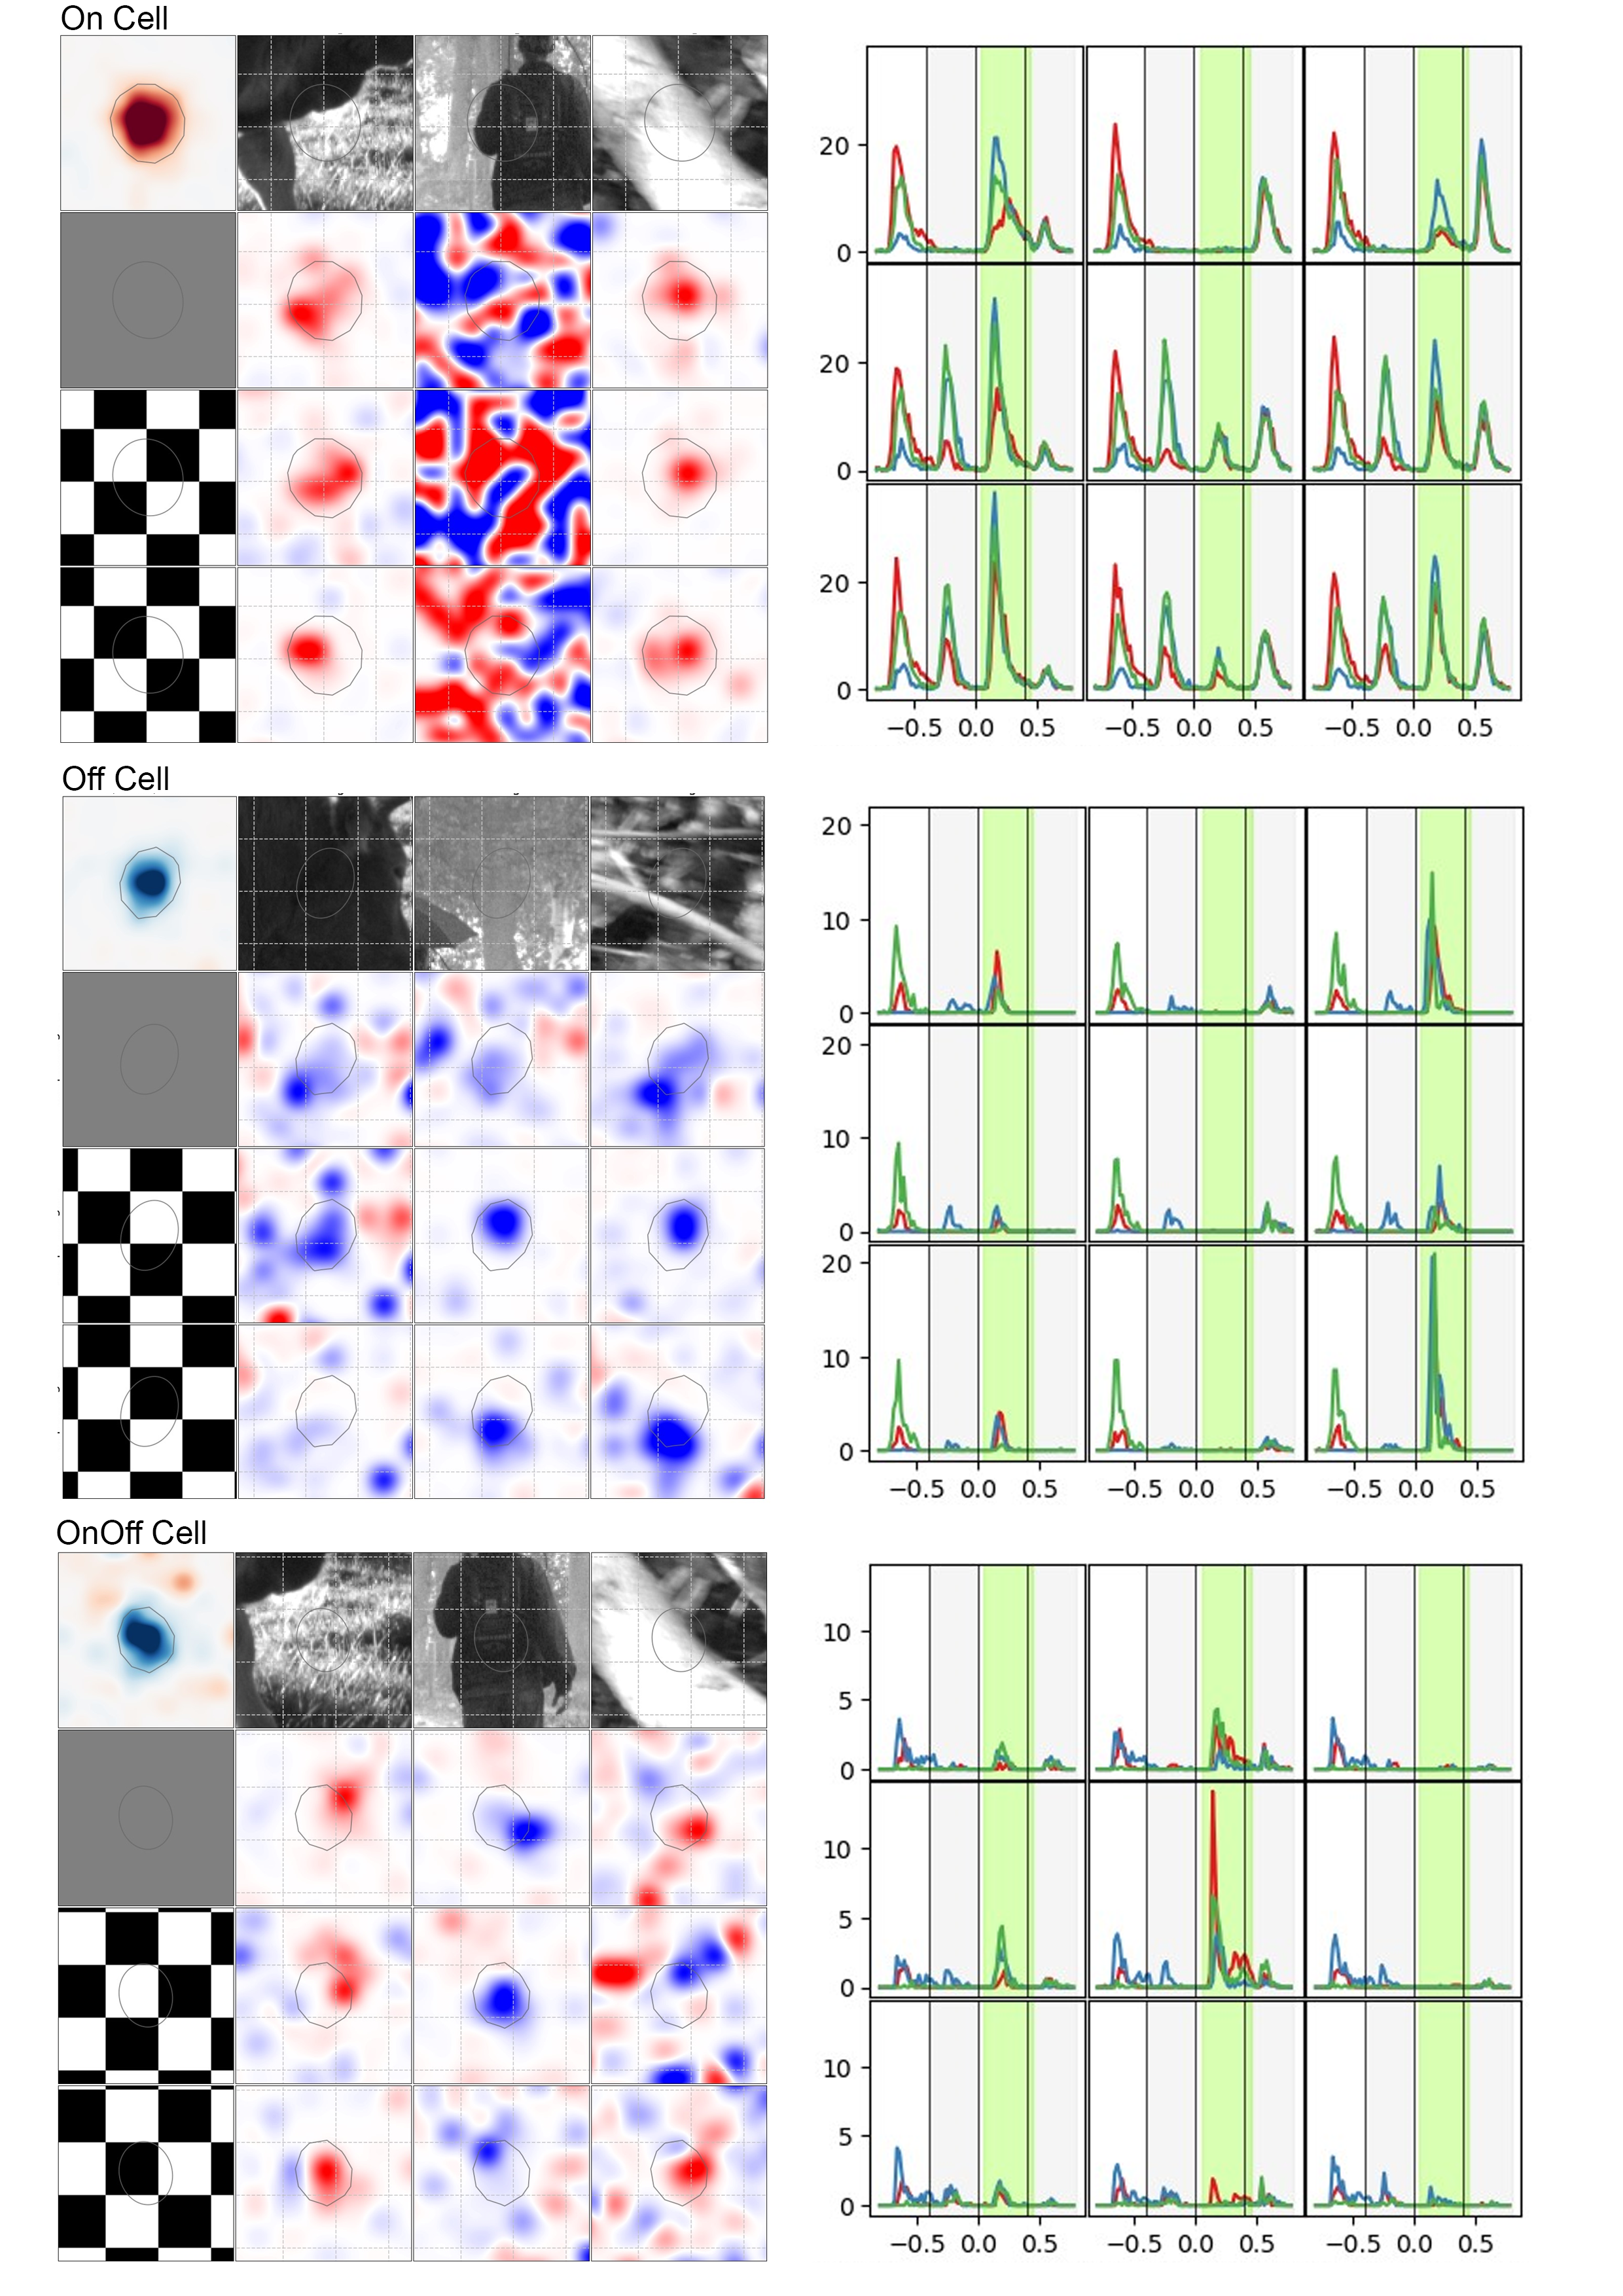
\includegraphics[width=0.8\textwidth]{pics/ExamplePSTHLSTA.png}
    \caption{\textbf{Temporal and spatial aspects of the response depend on
            previous light patterns: some
            exemplary RGCs.} \small	   \textbf{Left} Local Spike Triggered
        Average (LSTA), the average of the
        perturbation checkerboard patterns weighted by the number of spikes
        they
        evoked. Here we centered the view on the RGC receptive field and
        smoothed the
        LSTA using exponential tuning and spatial interpolation. We also
        display the STA in the top-left corner.
        \textbf{Right} Poststimulus time histograms
        (PSTH) are
        histograms of the times at which neurons fire.
        The disposition of the graph follows the same pattern as on the left.
        In each plot, the time
        bins in
        grey corresponds to the display of an adaptation pattern while time
        bins
        in
        white natural images.
        The time axis is centered on the moment when the current natural image
        is displayed. So in order the four rectangles are the previous natural
        image,
        current adaptation pattern, current natural image, and next adaptation
        pattern.
        The area highlighted in yellow corresponds to the 400 ms windows over
        which
        spikes are integrated to compute the LSTA.
        Each color corresponds to a different 'previous natural image'
        displayed 800ms before the current natural image.}
    \label{fig:CellExample}
\end{figure}

\textbf{Can a convolutional neural network model account for this dependence?}
We trained a convolutional neural network (CNN) model to predict the RGC
response to natural images. We hope to infer some of the governing
non-linearities in the recorded RGC. We expect the CNN model to have
good test performance on clips using the gray adaptation since it is trained on
such data However it's unclear how it will generalize to the other two
adaptation patterns. Additional divisive dynamics such as gain control would
have to be added to the model. More on model design can be found in Methods and
Appendix.

Here, we will show the results obtained from one of our models on one single
cell.
First, as we expected, the model predicted the clip using the gray adaptation
better and mostly failed in the other two cases (Figure
\ref{fig:CNNResults}.a). Notice that in most cases it
did predict a response but did not account for the new delay.
This hints at temporal dynamics being not well encoded in the CNN model.

However, test performances are not enough to validate a model that can be used
to build a hypothesis on the retinal code. We also have to make sure that the
model learns its filters to look like those of retinal cells. In the subunit,
we expect a center/surround spatial filter with a biphasic temporal filter. In
the RGC, we expect a localized receptive field, preferentially with a
center/surround spatial filter with a biphasic temporal filter. As shown in
Figure \ref{fig:CNNResults}.b, while the chosen model has a localized RGC
receptive field
with a slightly biphasic temporal filter, it lacks a clear surround in the
filter
of its subunits. As a consequence of the filters being too small, there are
large discontinuities on the border of the subunit filters that are not
desirable.
The structure of the filters is influenced by the L1 and L2 regularization that
are difficult to find tuned.

Finally, we would like to know if the CNN model can predict the displacement of
the LSTA observed before. We computed the LSTA as the average gradient of the
model over the frame of the stimulus that contained the natural image. This computation method is still in development. It seems
that the current model is not able to predict this displacement (Figure
\ref{fig:CNNResults}.c). This could
indicate that it structurally can't learn them, which would go in favor of
extending the model with more complex temporal dynamics such as gain control.
But it could also mean that the model was not properly trained.

\begin{figure}
    \centering
    \vspace*{-3cm}
    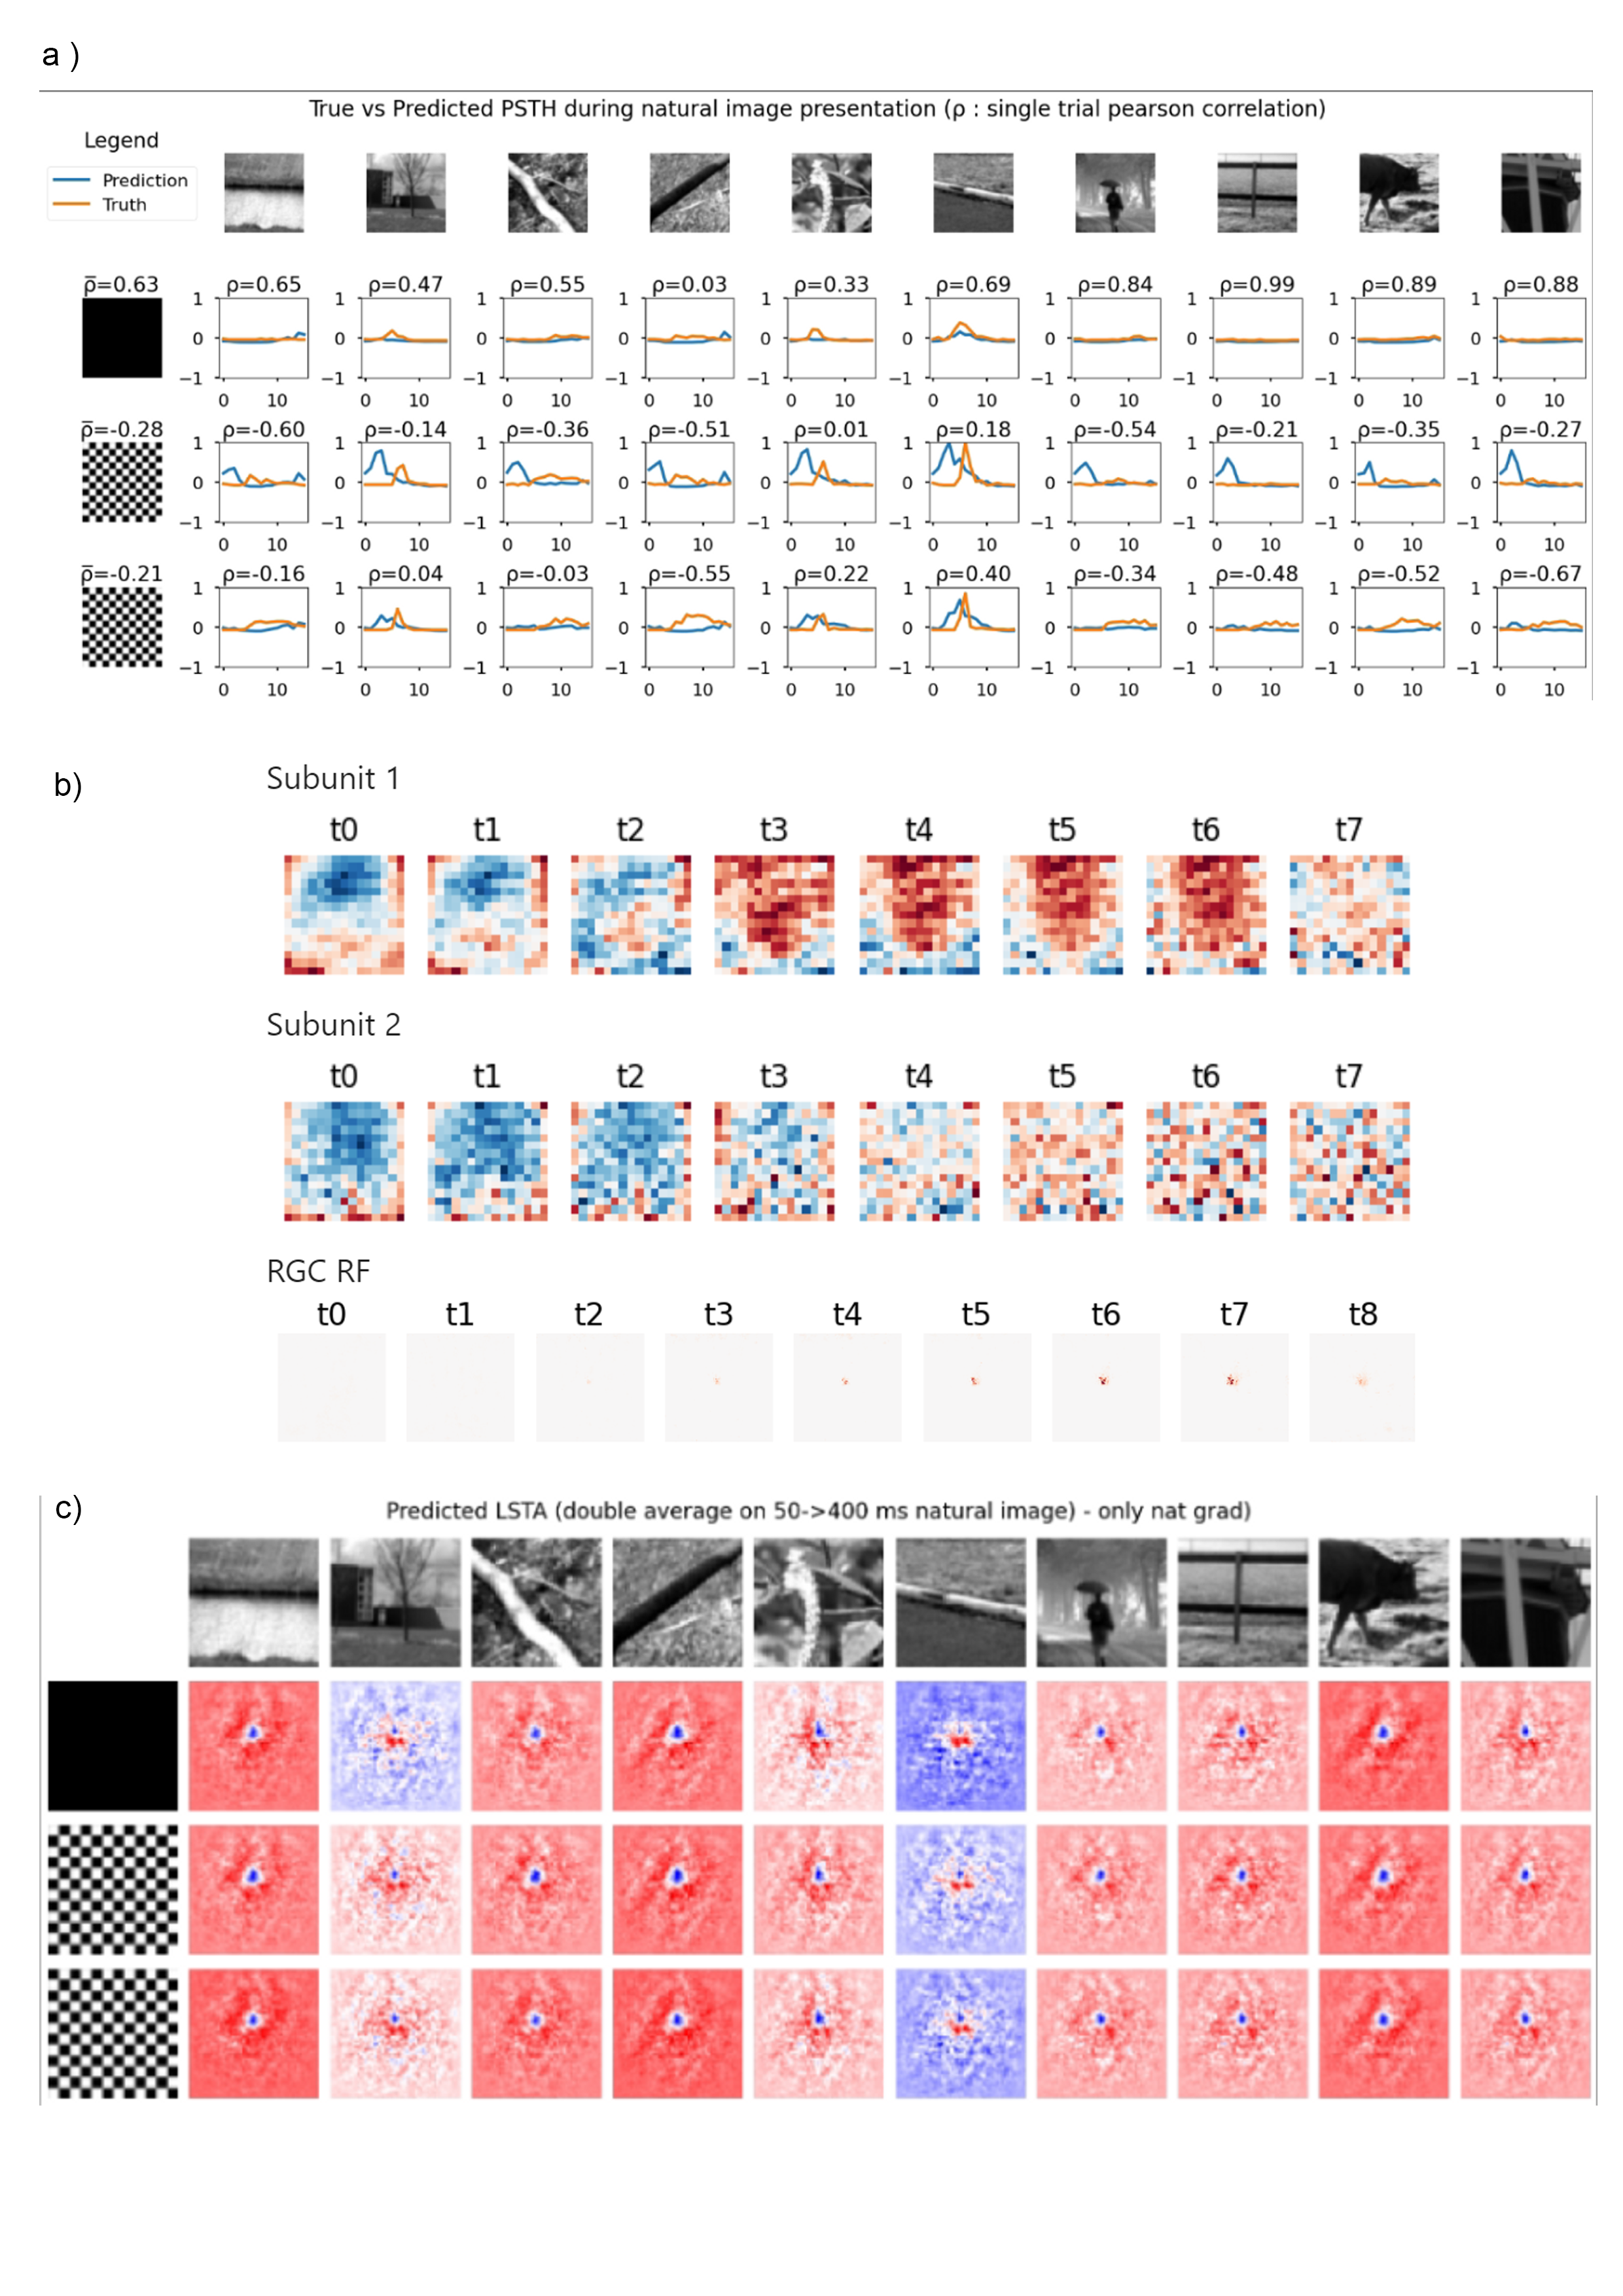
\includegraphics[width=\textwidth]{pics/CNNResults.png}
    \caption{\textbf{Resluts from the CNN model.} \textbf{a.} Single trial
        correlation $\rho$ performance
        of the CNN model on the three different adaptation patterns (see
        Methods). The model
        was
        trained on the gray adaptation pattern. \textbf{b.} Filters of the
        subunits and
        RGCs of the CNN model. \textbf{c.} LSTA computed from the CNN model.}
    \label{fig:CNNResults}
\end{figure}

\clearpage

\section{Conclusion}\label{sec:Conclusion}

% Summary
% Adaptation depends on previous patterns
We observed that during natural image stimulation, many ganglion cells change
their selectivity for different parts of the images depending on previous light
patterns.

% Modeling and Simulation
We combined large-scale recordings of RGC responses to natural movie
stimulations with CNN-based modeling to investigate such mechanisms of fast
contrast adaptation in the retina.
% Well I don't really have the rest to say here since it's not done

% Interplay of different subunit pathways
Under realistic regularization constraints, the CNNs learned a structure
similar to retinal pathways, where a ganglion cell activation is the result of
a pooling of local subunits of different types in a specific area in space, the
ganglion cell receptive field.

% Neural cells encode spatio-temporal features of natural scenes
Our result supports the idea that retinal ganglion cells encode both
spatial and temporal features of natural scenes on a local scale.
Previous works have described those features to be encoded as features of the
retinal response (latency, firing rate). We might be able to support this
theory with further comparison of measured responses with predicted responses
of
our model.

% Future Directions

Our work in the following months should take multiple directions. First, we are
investigating how more complex models perform on the prediction of LSTA (see
Annexe 1).
Second, we want to study if adding divisive non-linear temporal
dynamic in the subunits could help take the effect of the adaptation images
into
account (see Annexe 2).
Third, we would be interested to see if the LSTA adaptation is only dependent
on the local luminance of the adaptatio images or also on the local temporal
contrast. To do that we could add flickering of different speed to the black
and white checks.

% Comparative analysis

% Utility of measurements tools
Maheswaranathan and colleagues \citep{maheswaranathan_interpreting_2023} have
recently
been able to predict different aspect of encoding in the retina using deep
comvolutional network. In comparison, our experimental approach of estimating
the LSTA allow a direct comparison from the model to the data. Classical
estimation of performance can't describe what is missed in the prediction,
while our qualitative comparison might be able to.

% The what, why and how the retina
% I think it's and accessible illustration of the main questions regarding the retinal code
The modeling of retinal responses to natural stimuli has improved our
understanding of complex retinal processing. In a recent review, Karamanlis and
colleagues \citep{} [ADD TO BIB], suggested three perspectives of study on the
retinal
encoding of natural scenes: The circuit perspective ('How is the retinal code
implemented?'), the normative perspective ('Why is it complimented this way?)
and the coding perspective ('What is the code used by the retina?'). In this
work, we focused on the 'what' for now. By exploring the response of the retina
to a portion of
the spatio-temporal stimuli space we can gain insight into the code used by the
retina on that subspace. To explore further the 'how' perspective, one would
need to study how the different known types of cells in the retina participate
in that encoding. This poses the challenge of bridging the typing of cells from
functional and anatomical perspectives.
The normative perspective has also been explored using deep CNNs with
anatomically realistic constrained. It is likely that species with simpler
cortical circuitry, as mice, have a stronger need for upstream feature
extraction, in the retina [ADD CITE]. In opposition, species with computationally powerful
cortexes such as primates can deal with more faithful and linear
representations
of the visual inputs.

% Your references go at the end of the main text, and before the
% figures.  For this document we've used BibTeX, the .bib file
% scibib.bib, and the .bst file Science.bst.  The package scicite.sty
% was included to format the reference numbers according to *Science*
% style.

%BibTeX users: After compilation, comment out the following two lines and paste in
% the generated .bbl file. 

\bibliography{biblio}

% \bibliographystyle{Science}


%Here you should list the contents of your Supplementary Materials -- below is an example. 
%You should include a list of Supplementary figures, Tables, and any references that appear only in the SM. 
%Note that the reference numbering continues from the main text to the SM.
% In the example below, Refs. 4-10 were cited only in the SM.     

\section*{Supplementary materials}

\begin{figure}[ht]
    \centering
    \includegraphics[[width=\textwidth]]{pics/GCModelDiagram.png}
    \caption{\textbf{Quick sketch of a gain control LNLN model.} Each bipolar
        cell is
        composed of a linear spatial filter that selectively responds to part
        of the scene,
        a non-linear activation function, and a gain control mechanism that
        scale its output
        depending on past events. They all converge into on bipolar cell
        (forming its receptive field)
        of which output is also modeled using a non-linear function.}
    \label{fig:LNLN}
\end{figure}

\clearpage

\end{document}